% Auriga theme
% find the most up-to-date version here: https://github.com/anishathalye/auriga

\documentclass[14pt,aspectratio=169]{beamer}
\usepackage{pgfpages}
\usepackage{fancyvrb}
\usepackage{graphicx}
\usepackage[
backend=biber,
style=alphabetic,
citestyle=authoryear
]{biblatex}

\addbibresource{references.bib} %Imports bibliography file

%\ifnotes
%\setbeamertemplate{note page}[plain]
%\setbeameroption{show notes on second screen=right}
%\fi

\usetheme{auriga}
\usecolortheme{auriga}

% define graphics path
\graphicspath{{./figures/}}

% define some colors for a consistent theme across slides
\definecolor{red}{RGB}{181, 23, 0}
\definecolor{blue}{RGB}{0, 118, 186}
\definecolor{gray}{RGB}{146, 146, 146}

\title{PFR of Dispatched Generation on 25/08/2018}

\author{Excludes generation enabled for assisting FCAS}

%\author{\underline{Alyssa P. Hacker} \inst{1} \and Ben Bitdiddle \inst{2} \and Lem E. Tweakit \inst{2}}

%\institute[shortinst]{\inst{1} Some Institute \samelineand \inst{2} %Another Institute}

\begin{document}

{
  % rather than use the frame options [noframenumbering,plain], we make the
  % color match, so that the indicated page numbers match PDF page numbers
  \setbeamercolor{page number in head/foot}{fg=background canvas.bg}
  \begin{frame}
    \titlepage
  \end{frame}
}

\begin{frame}{Summary of Regional Frequencies}

  \begin{itemize}
    \item \textbf{QLD}
    \begin{itemize}
        \item exporting to NSW
        \item over frequency after AC separation from NSW (13:11:41.2)
    \end{itemize}
    \item \textbf{SA}
      \begin{itemize}
        \item initially under-frequency after QNI trip when connected to NSW-VIC
        \item within 5 seconds (13:11:46.8), Heywood trips resulting in AC separation of SA and NSW-VIC
            \begin{itemize}
                \item results in over-frequency
            \end{itemize}
        \end{itemize}
    \item \textbf{NSW-VIC}
        \begin{itemize}
            \item under-frequency following successive trips of QNI and Heywood
        \end{itemize}
  \end{itemize}

%   \note{
%     Here's a note for this slide.
%   }

\end{frame}

\begin{frame}{Observing Generator PFR}

  \begin{itemize}
    \item Data availability
    \begin{itemize}
        \item FCAS Causer Pays data (4 second frequency)
        \item NSW-VIC, SA, QLD regional frequency data (1 second frequency)
    \end{itemize}
    \item Data limitations
    \begin{itemize}
        \item communication delays and/or data processing in Causer Pays
            \begin{itemize}
                \item leads to 'lagged' response in data
                \begin{itemize}
                    \item determine if appropriate to apply leading adjustment across dataset
                \end{itemize}
            \end{itemize}
        \item sampling and/or data processing in Causer Pays
            \begin{itemize}
                \item under-sampling might hide true generator response
            \end{itemize}
    \end{itemize}
  \end{itemize}
\end{frame}
\begin{frame}{Observing Generator PFR}
\begin{itemize}
\item Steps
    \begin{enumerate}
        \item Determine if leading adjustment required for Causer Pays
        \item Identify generators scheduled for DI 13:10-13:15
        \item Isolate generators not providing assisting FCAS
        \begin{itemize}
            \item Observed response will reflect PFR of generator when operation in frequency-responsive mode is not mandatory
        \end{itemize}
        \item Use Causer Pays data to observe gen response over DI
    \end{enumerate}
  \end{itemize}
 
 \end{frame}
\begin{frame}{Summary of Observations}
\begin{itemize}
\itemsep0em
\item Data lag
\begin{itemize}
    \item inconsistency in data lag for one interconnector
    \item leading correction needed if interested in response magnitude rather than time?
    \item \textbf{no lag correction/leading applied to Causer Pays dataset}
\end{itemize}
\item Generator response
\begin{itemize}
    \item Predominantly no or withdrawn PFR for synchronous units
    \item No response from inverter-based renewables except for GPS
    \item Most interesting responses in SA and QLD where frequency deviation outside NOFB was sustained
\end{itemize}
\end{itemize}
 
 \end{frame}
\begin{frame}{Leading Adjustment - Interconnectors}

  \begin{columns}
    \begin{column}{0.6\linewidth}
    \begin{figure}[t]
        \vspace{-0.5cm}
        \centering
        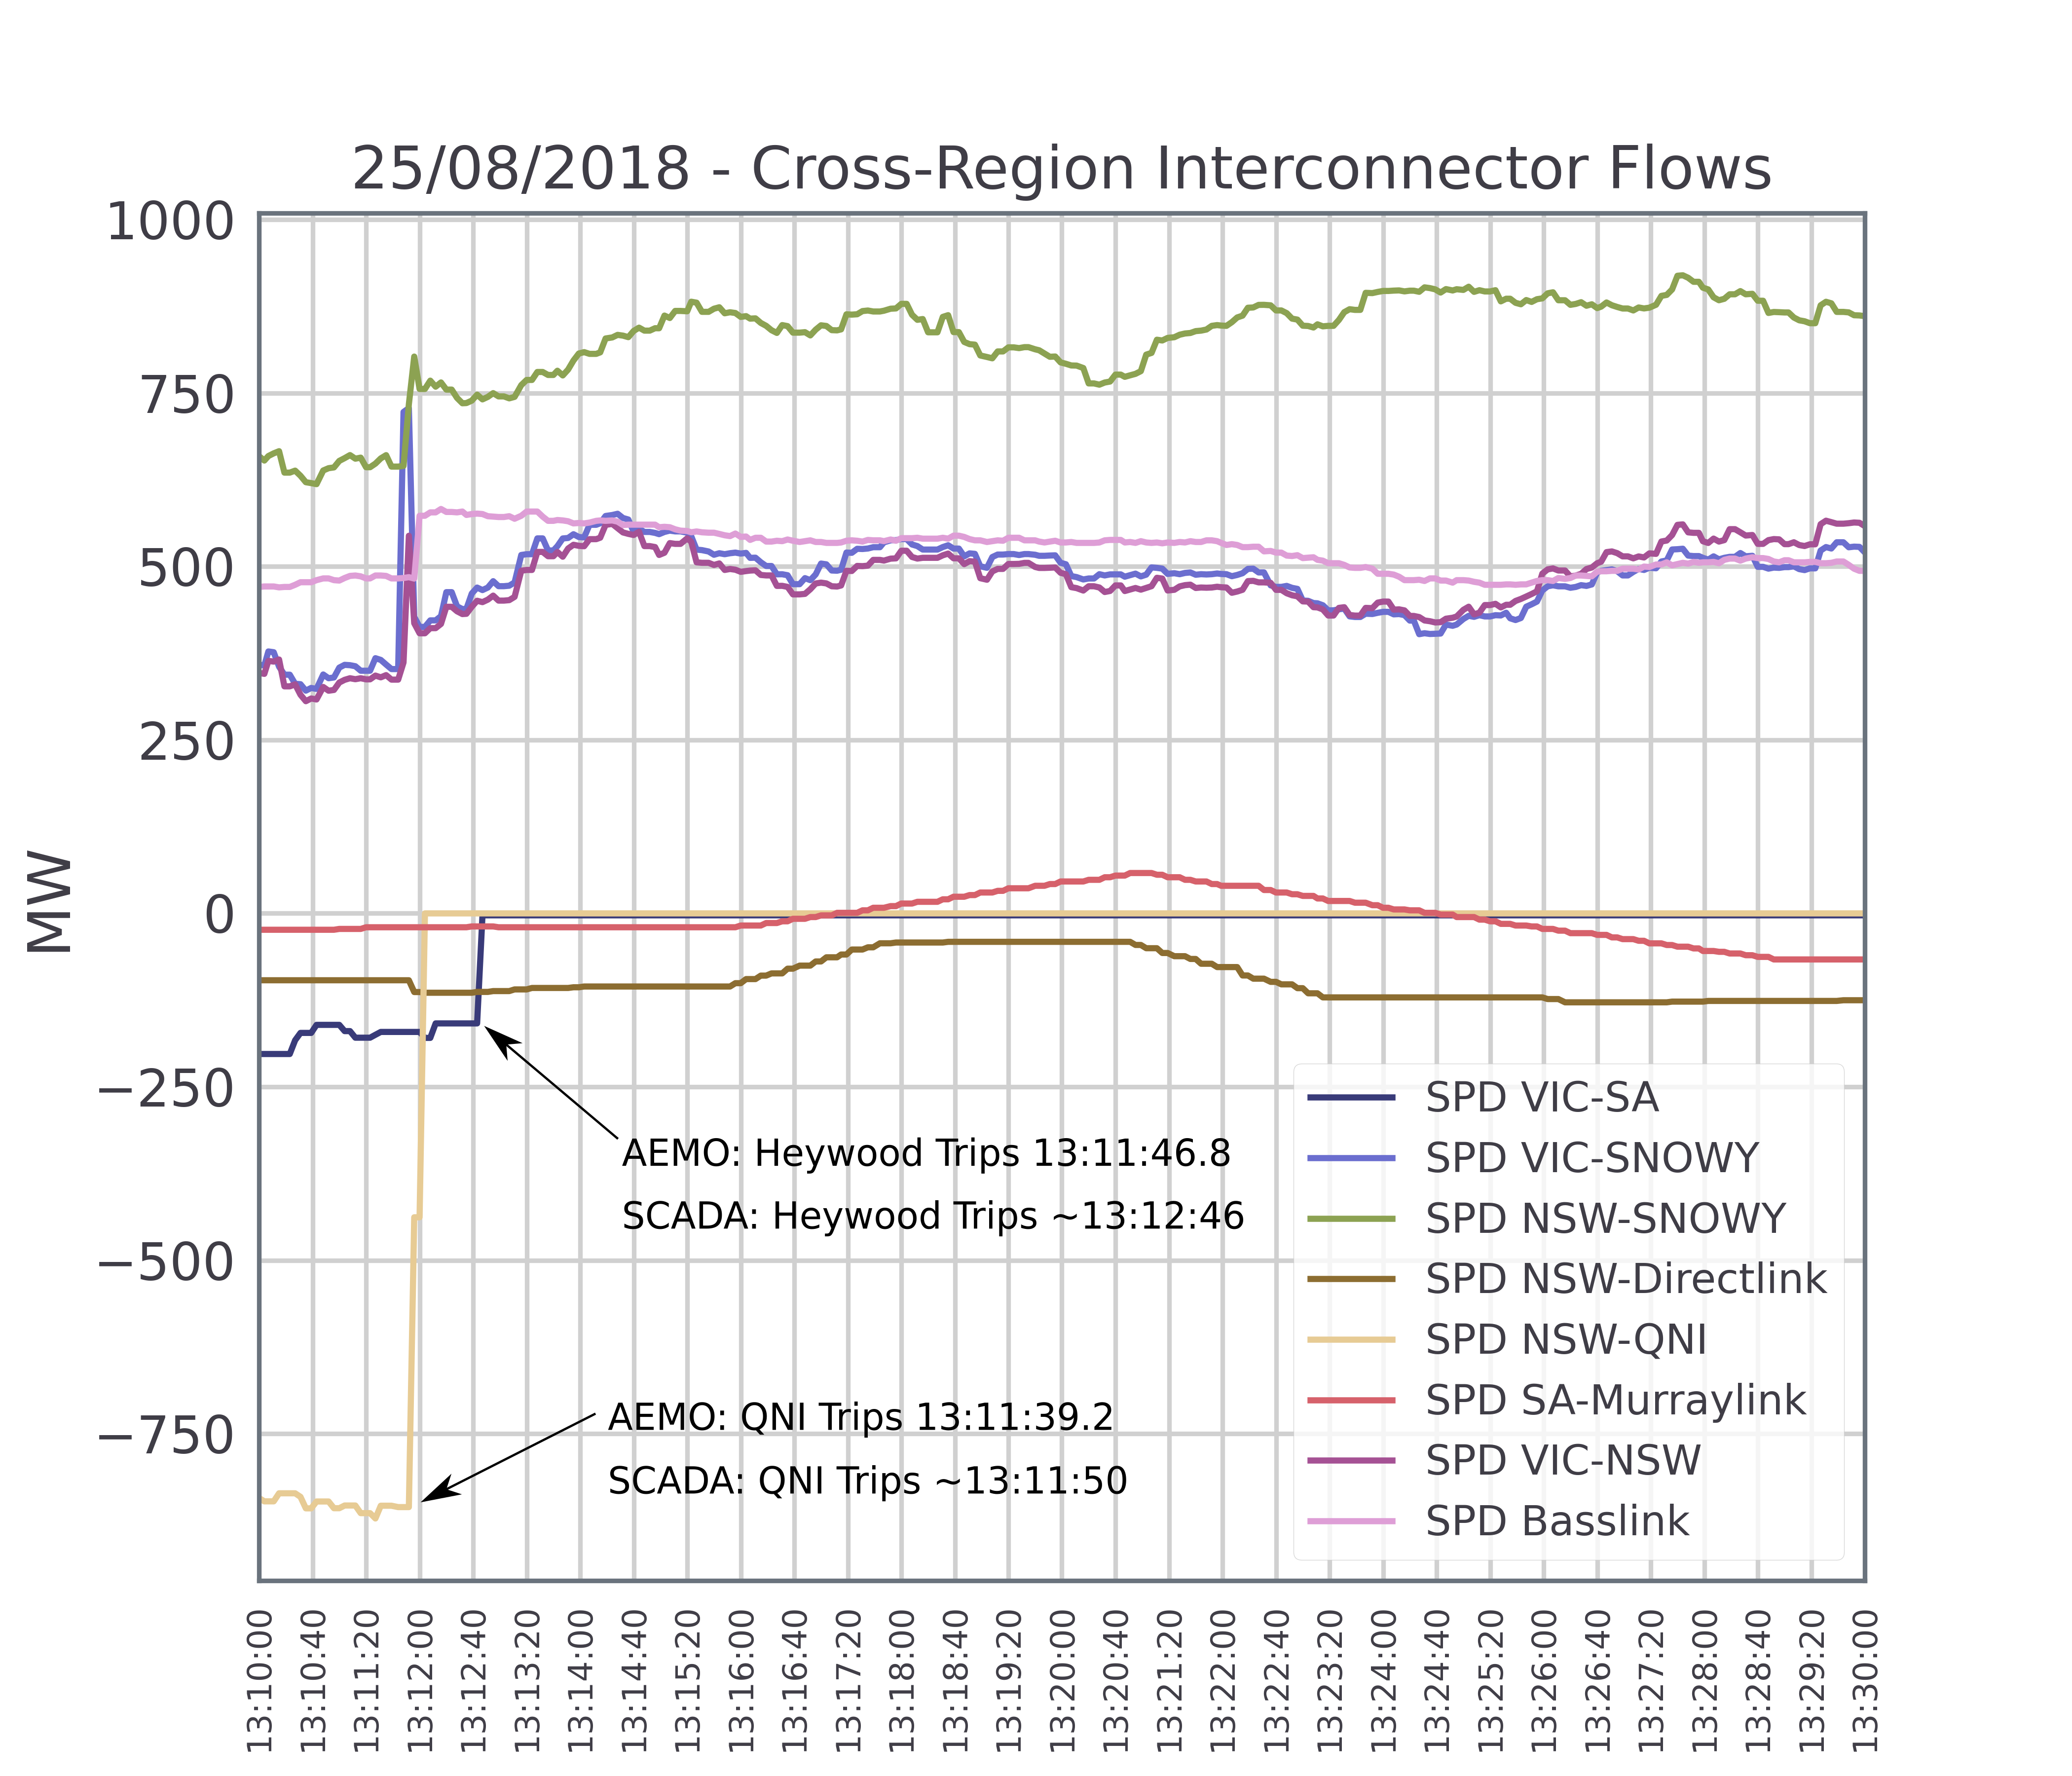
\includegraphics[width=\linewidth]{figures/interconnector_flows_annotated.png}
        \label{fig:intercon}
    \end{figure}
    \end{column}
    
    \begin{column}{0.4\linewidth}
    \begin{itemize}
        \item \textasciitilde10 second lag in the QNI trip
        \item \textasciitilde1 minute lag in Heywood trip in Causer Pays data
        \item Inconsistent lag
    \end{itemize}
    \end{column}
  \end{columns}

%  \note{
%     This slide has notes too.
%   }

\end{frame}

\begin{frame}{Leading Adjustment - Regional Frequencies}

  \begin{columns}
    \begin{column}{0.6\linewidth}
    \begin{figure}
    \centering
        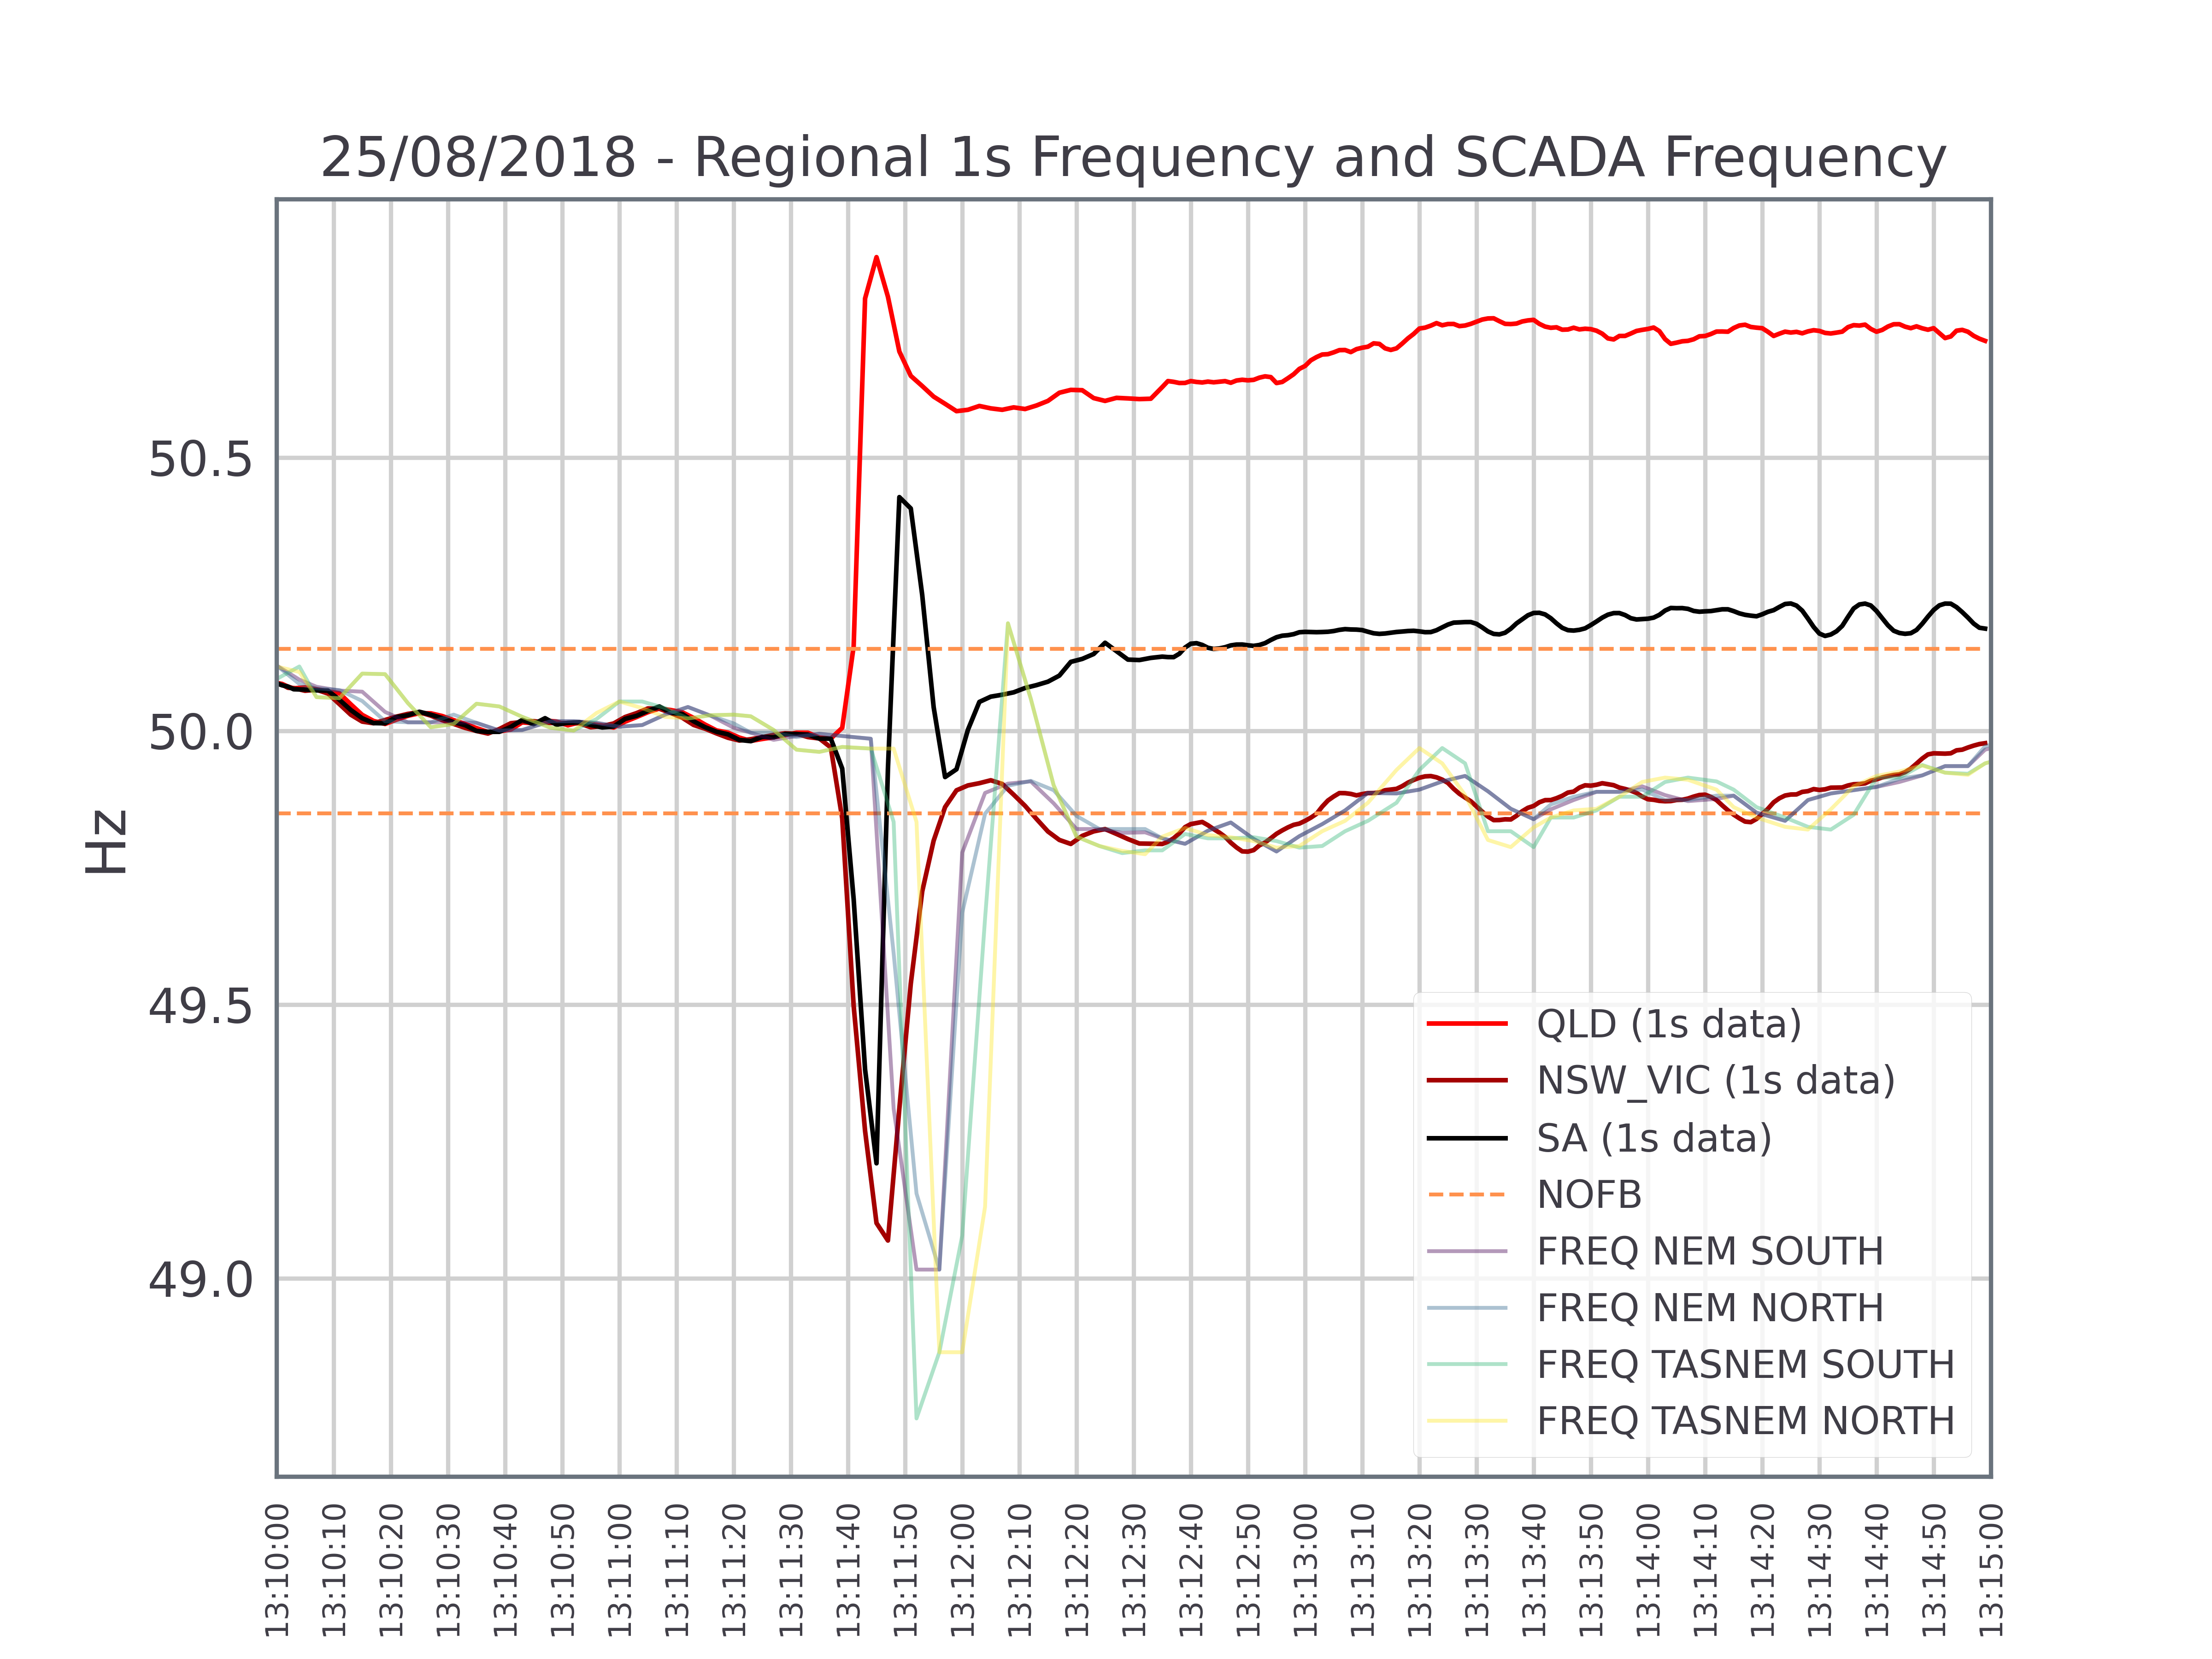
\includegraphics[width=\linewidth]{figures/regional_SCADA_frequencies.png}
        \label{fig:reg_freqs}
    \end{figure}
    \end{column}
    
    \begin{column}{0.4\linewidth}
    \begin{itemize}
        \item Regional frequency data consistent with AEMO's report
        \item Causer Pays data for NEM North and South appears to match NSW-VIC
            \begin{itemize}
                \item different nadir magnitude
                \item lag of 8-10 seconds
            \end{itemize}
    \end{itemize}
    \end{column}
  \end{columns}

%  \note{
%     This slide has notes too.
%   }

\end{frame}

\begin{frame}{Generator Response}
\begin{itemize}
\item Operating modes as described in \cite{Undrill2018}
    \begin{itemize}
        \item Droop mode or droop-dominated mode, where droop response is sustained. Load controller does not interfere,
        \item Prescheduled output mode without frequency bias, where initial PFR withdrawn by load controller to scheduled load setpoint
        \item Prescheduled output mode with frequency bias, where load controller moves unit to offset scheduled load setpoint after iniial PFR. Offset dependent on system frequency
        \item AGC mode
        \item Non-responsive mode
    \end{itemize}
\end{itemize}
\end{frame}
\begin{frame}{Generator Response - QLD Subcritical Coal }

\begin{figure}
    \centering
    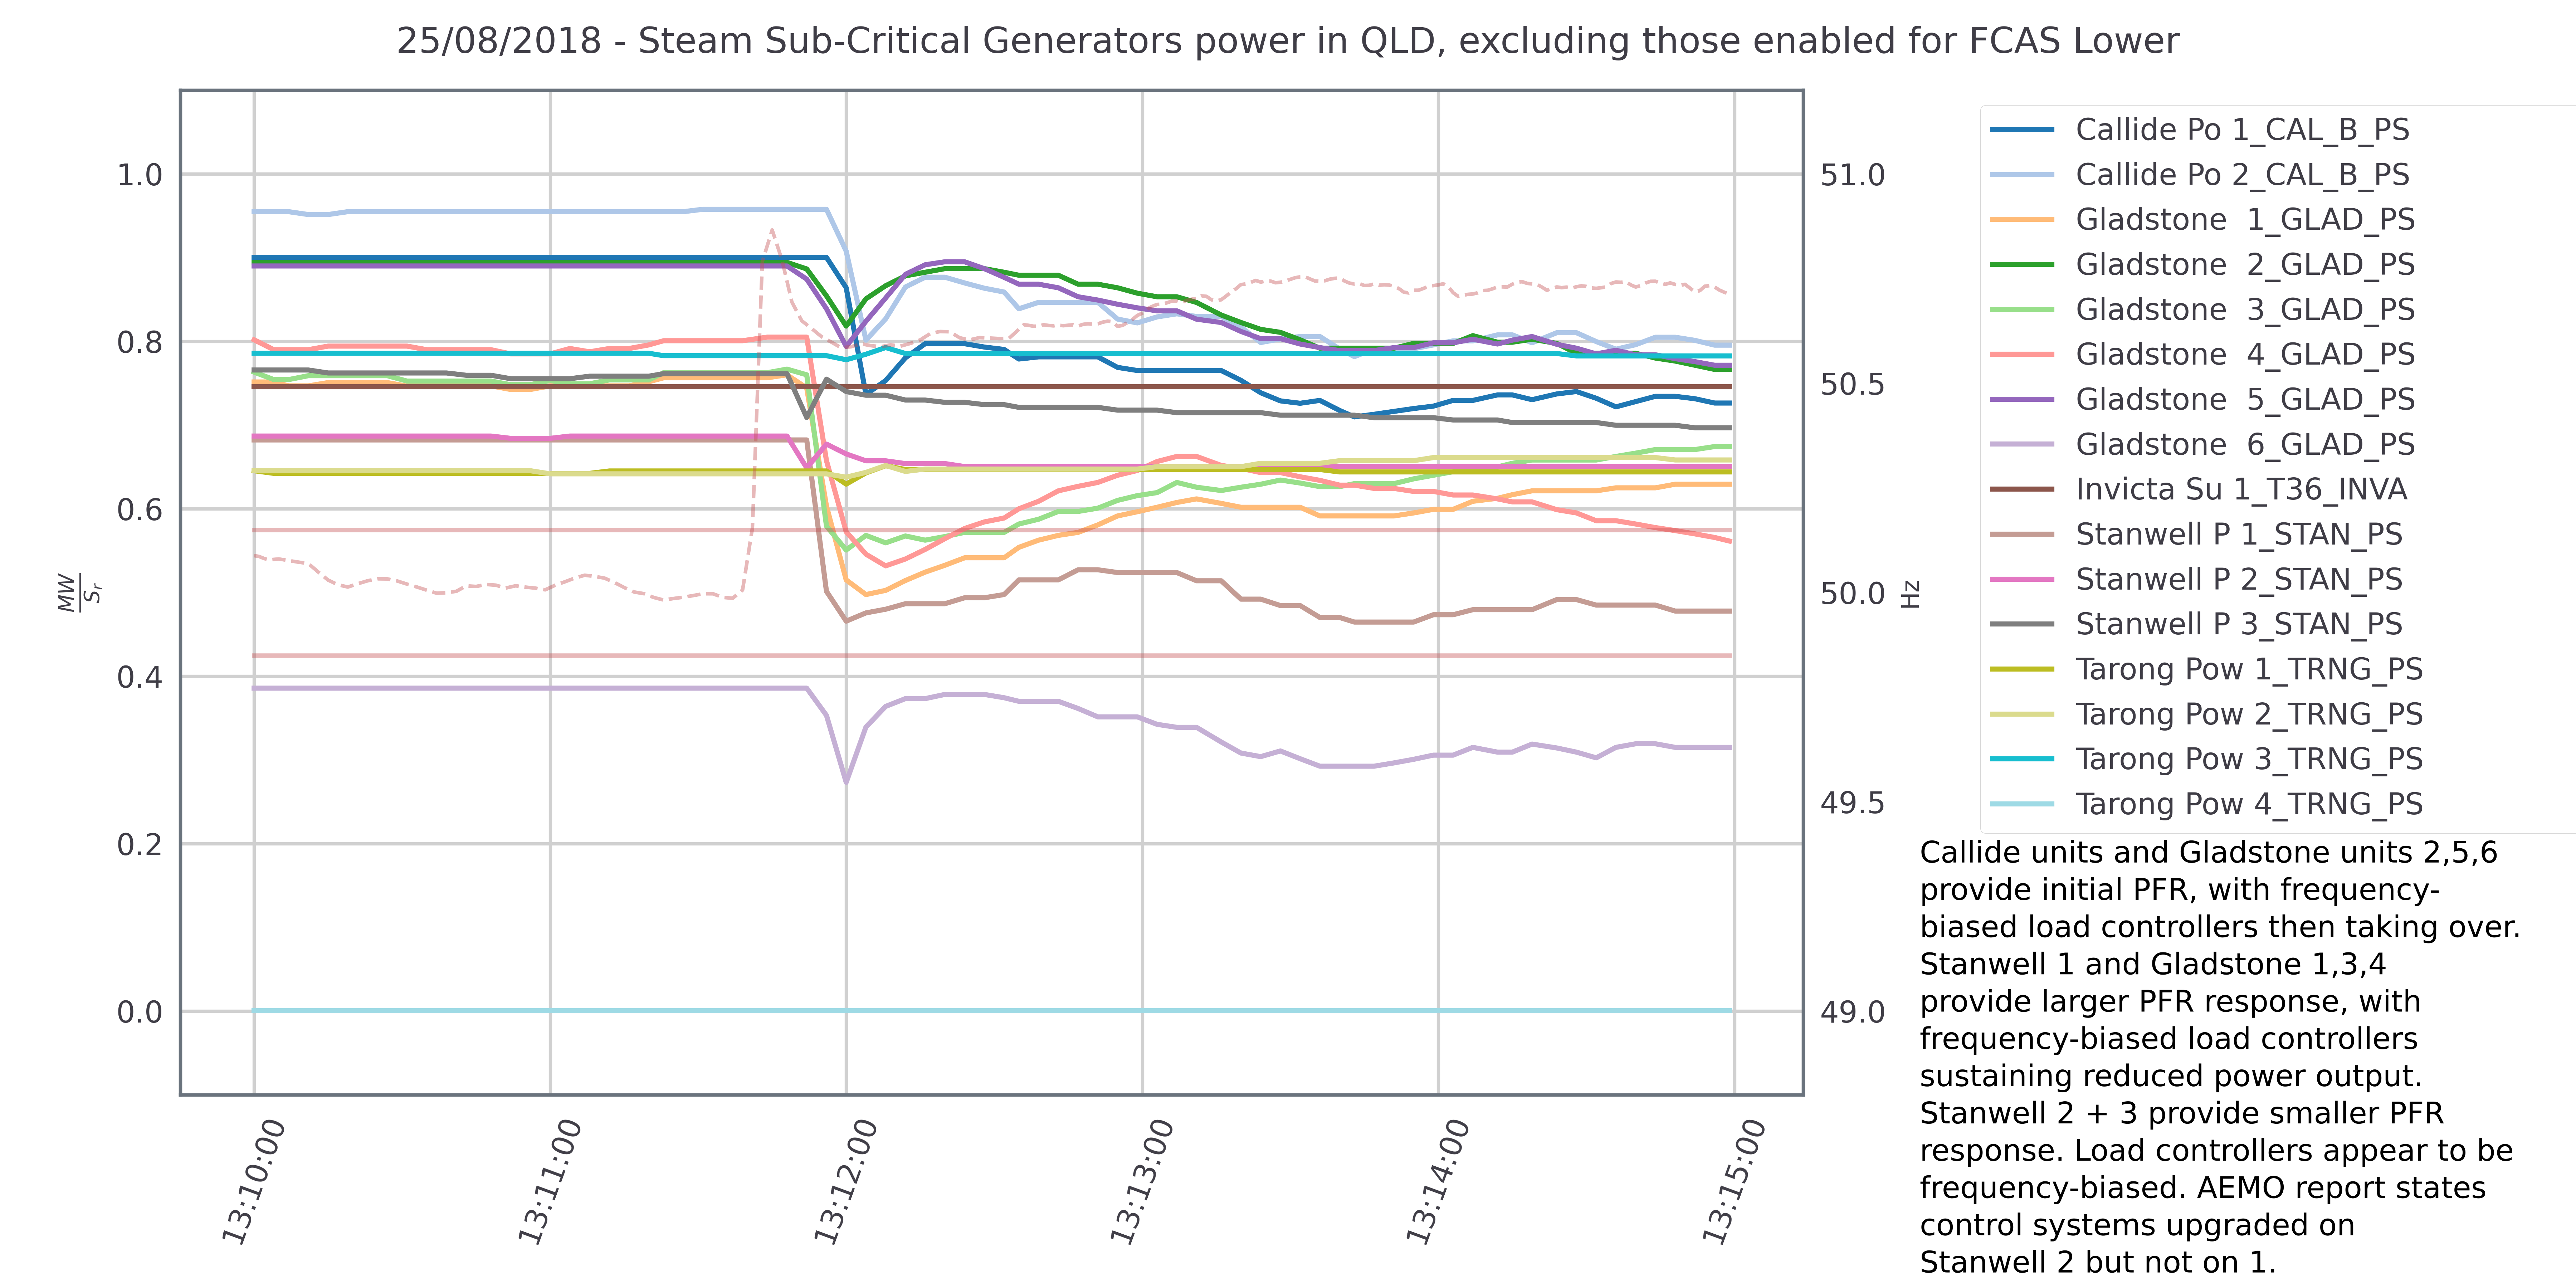
\includegraphics[width=\linewidth]{figures/QLD_Steam Sub-Critical_PU_annotated.png}
    \label{fig:qld_sub}
\end{figure}

%  \note{
%     This slide has notes too.
%   }

\end{frame}

\begin{frame}{Generator Response - QLD Supercritical Coal }

\begin{figure}
    \centering
    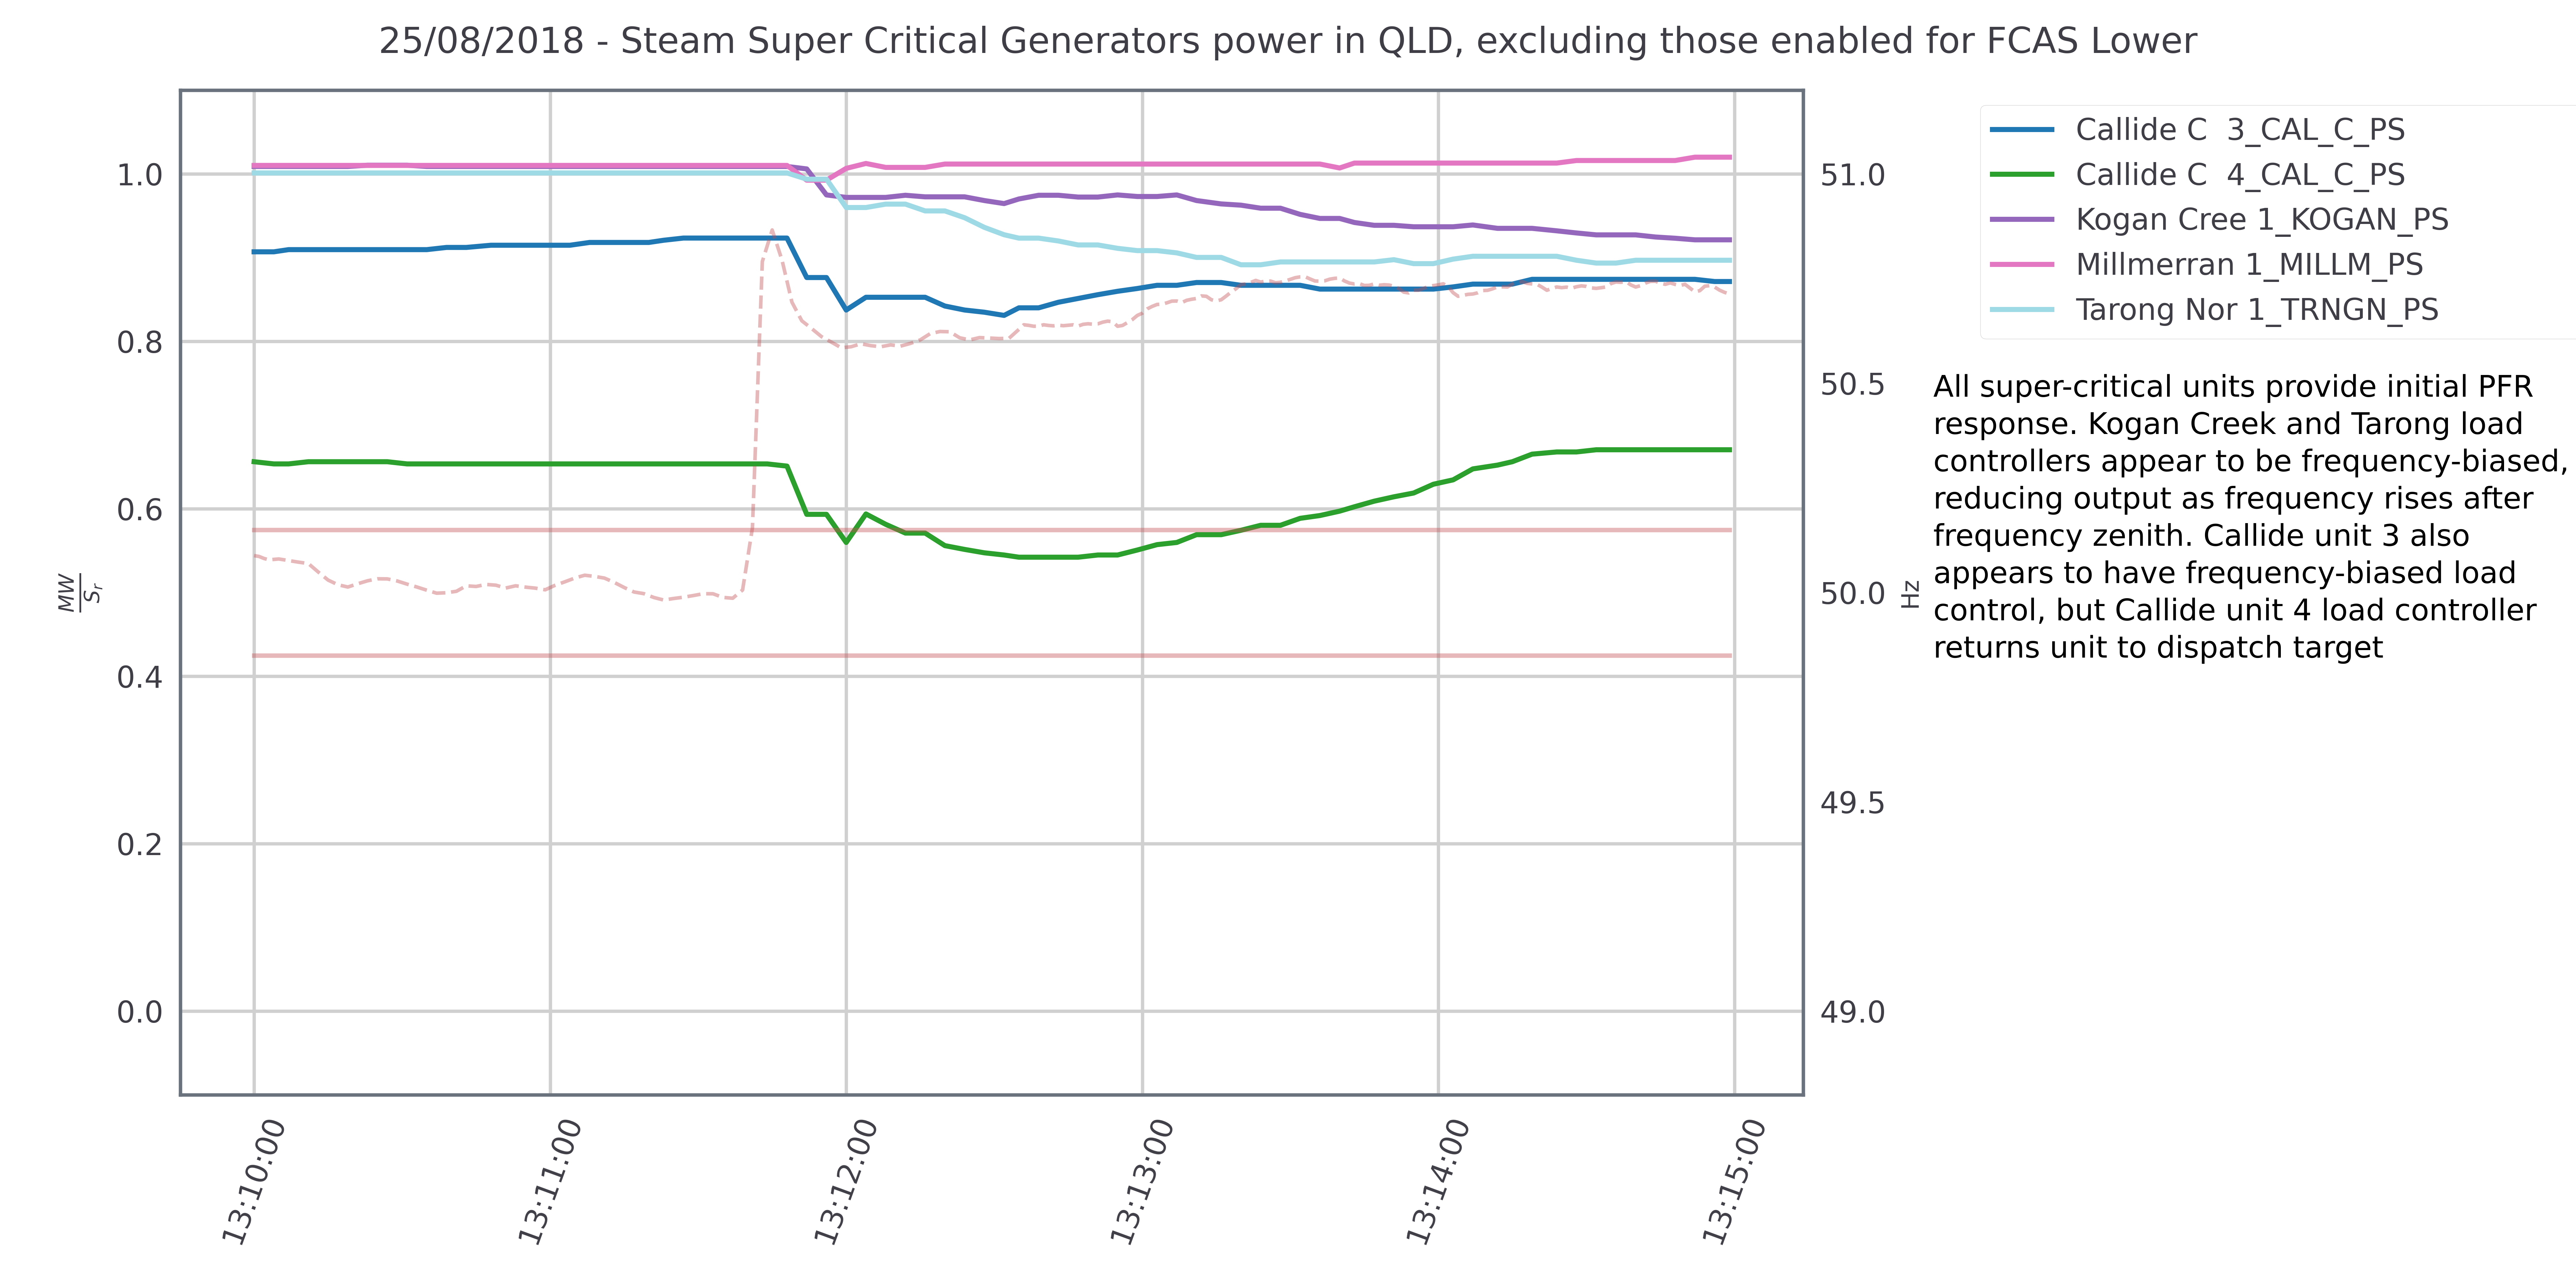
\includegraphics[width=\linewidth]{figures/QLD_Steam Super-Critical_PU_annotated.png}
    \label{fig:qld_super}
\end{figure}

%  \note{
%     This slide has notes too.
%   }

\end{frame}

\begin{frame}{Generator Response - SA Wind}

\begin{figure}
    \centering
    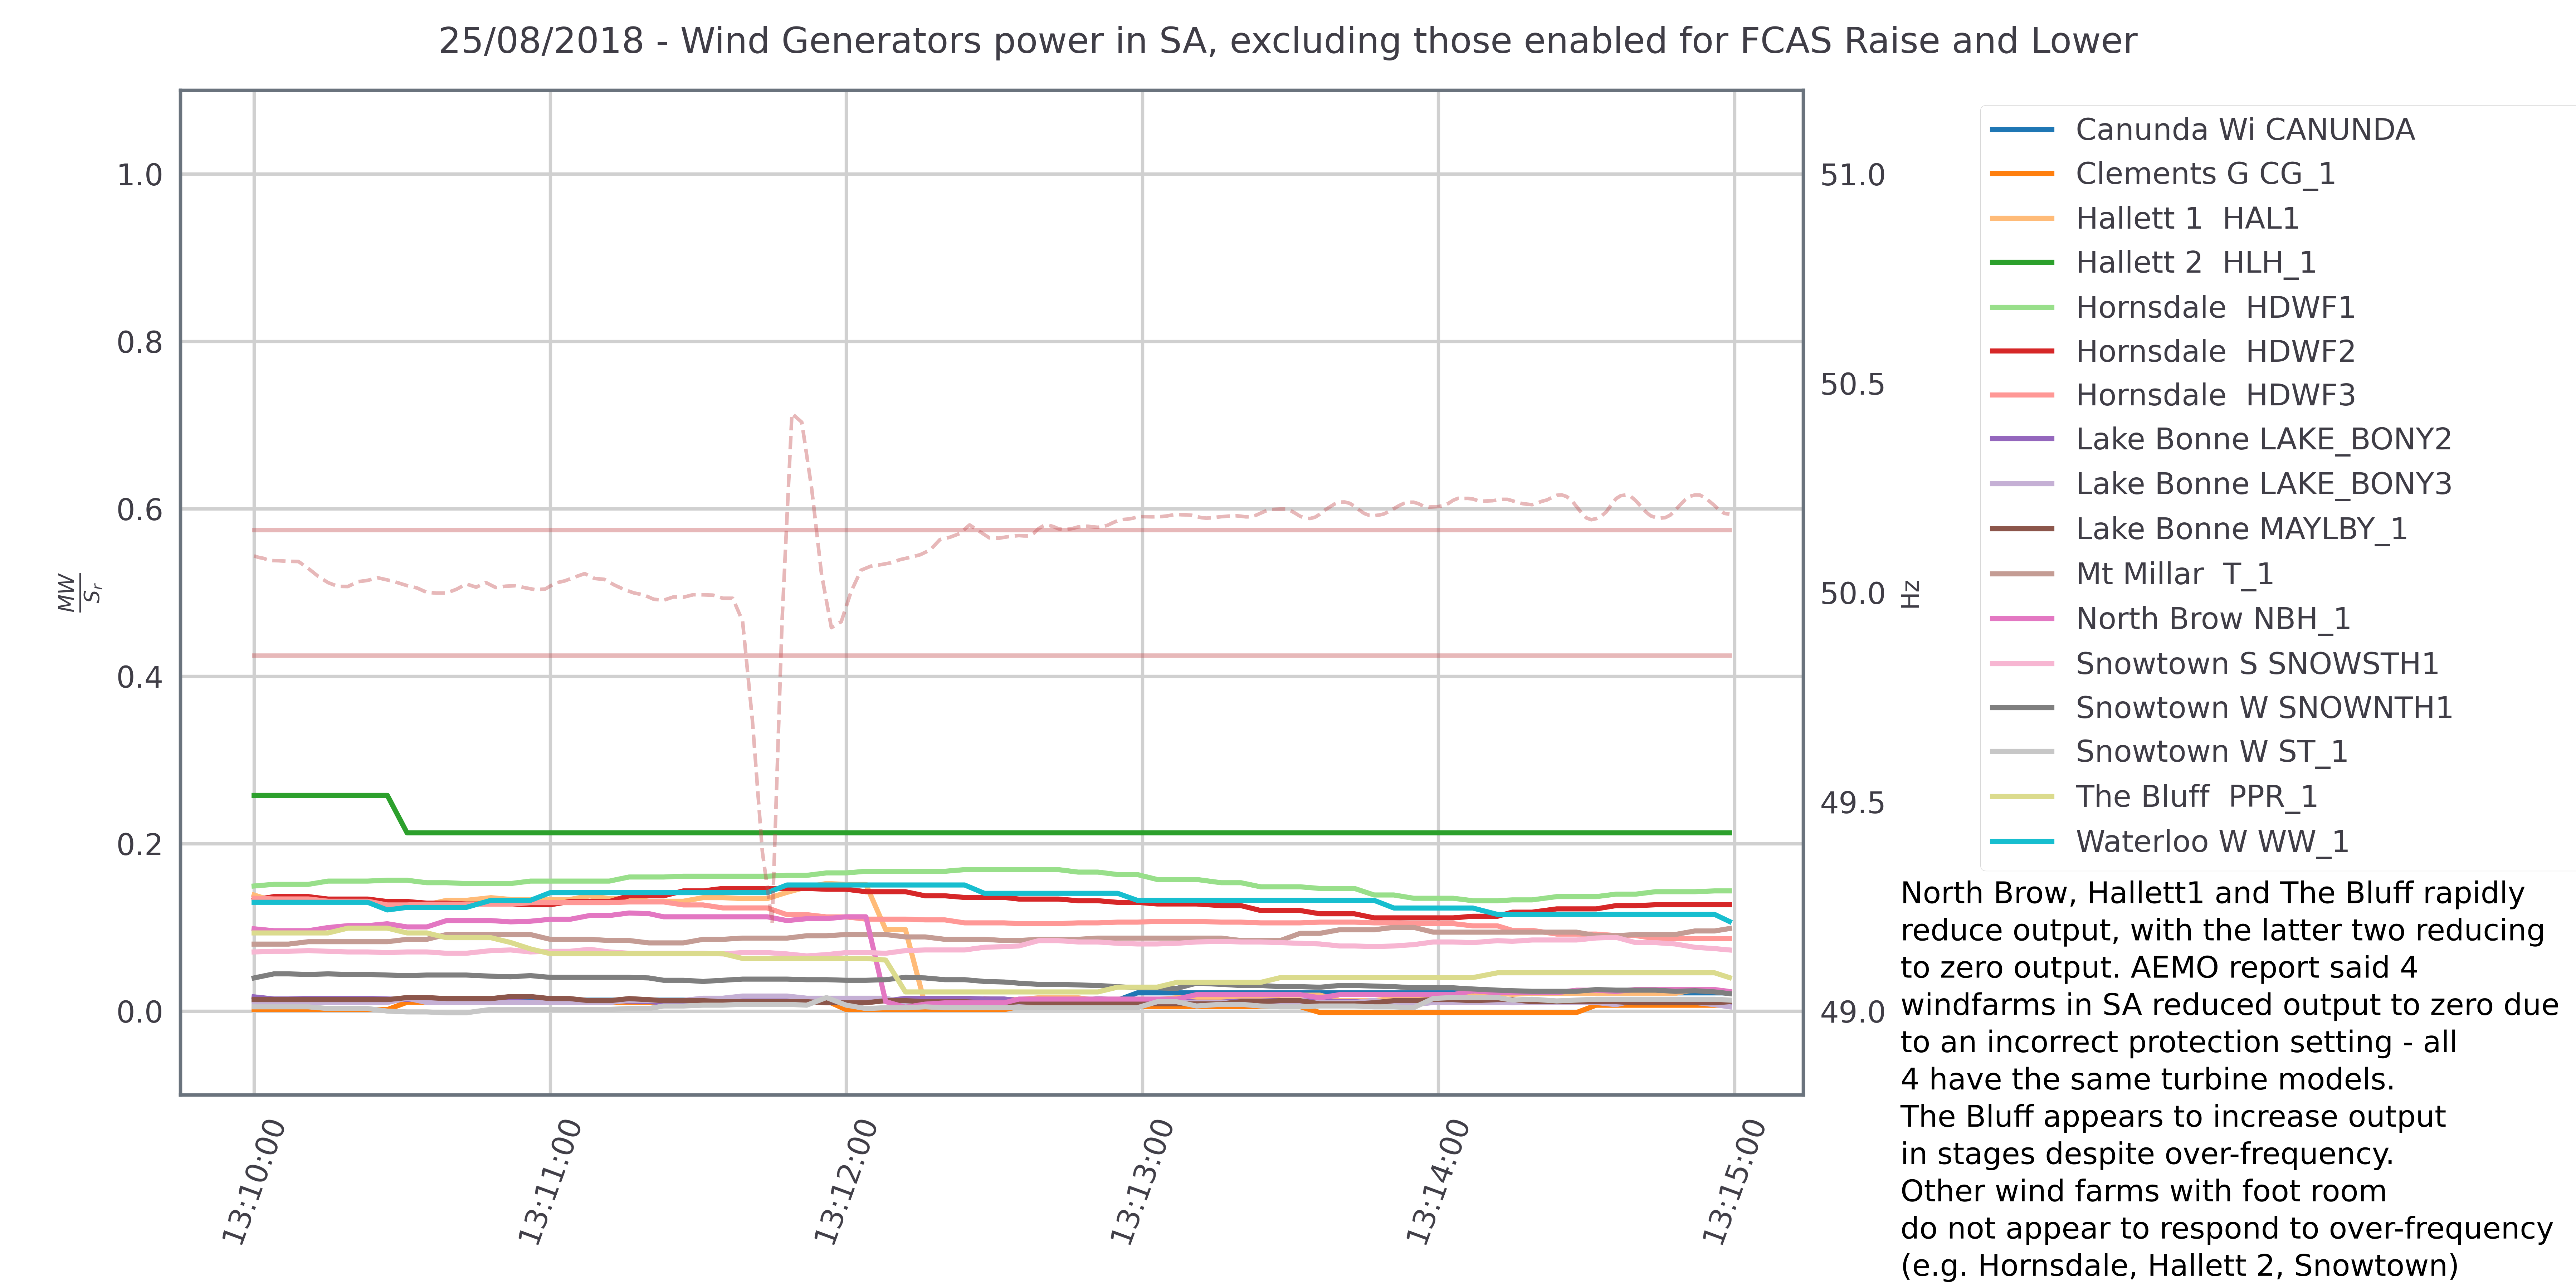
\includegraphics[width=\linewidth]{figures/SA_Wind_PU_annotated.png}
    \label{fig:sa_wind}
\end{figure}

%  \note{
%     This slide has notes too.
%   }

\end{frame}

\begin{frame}{Generator Response - QLD PV}

\begin{figure}
    \centering
    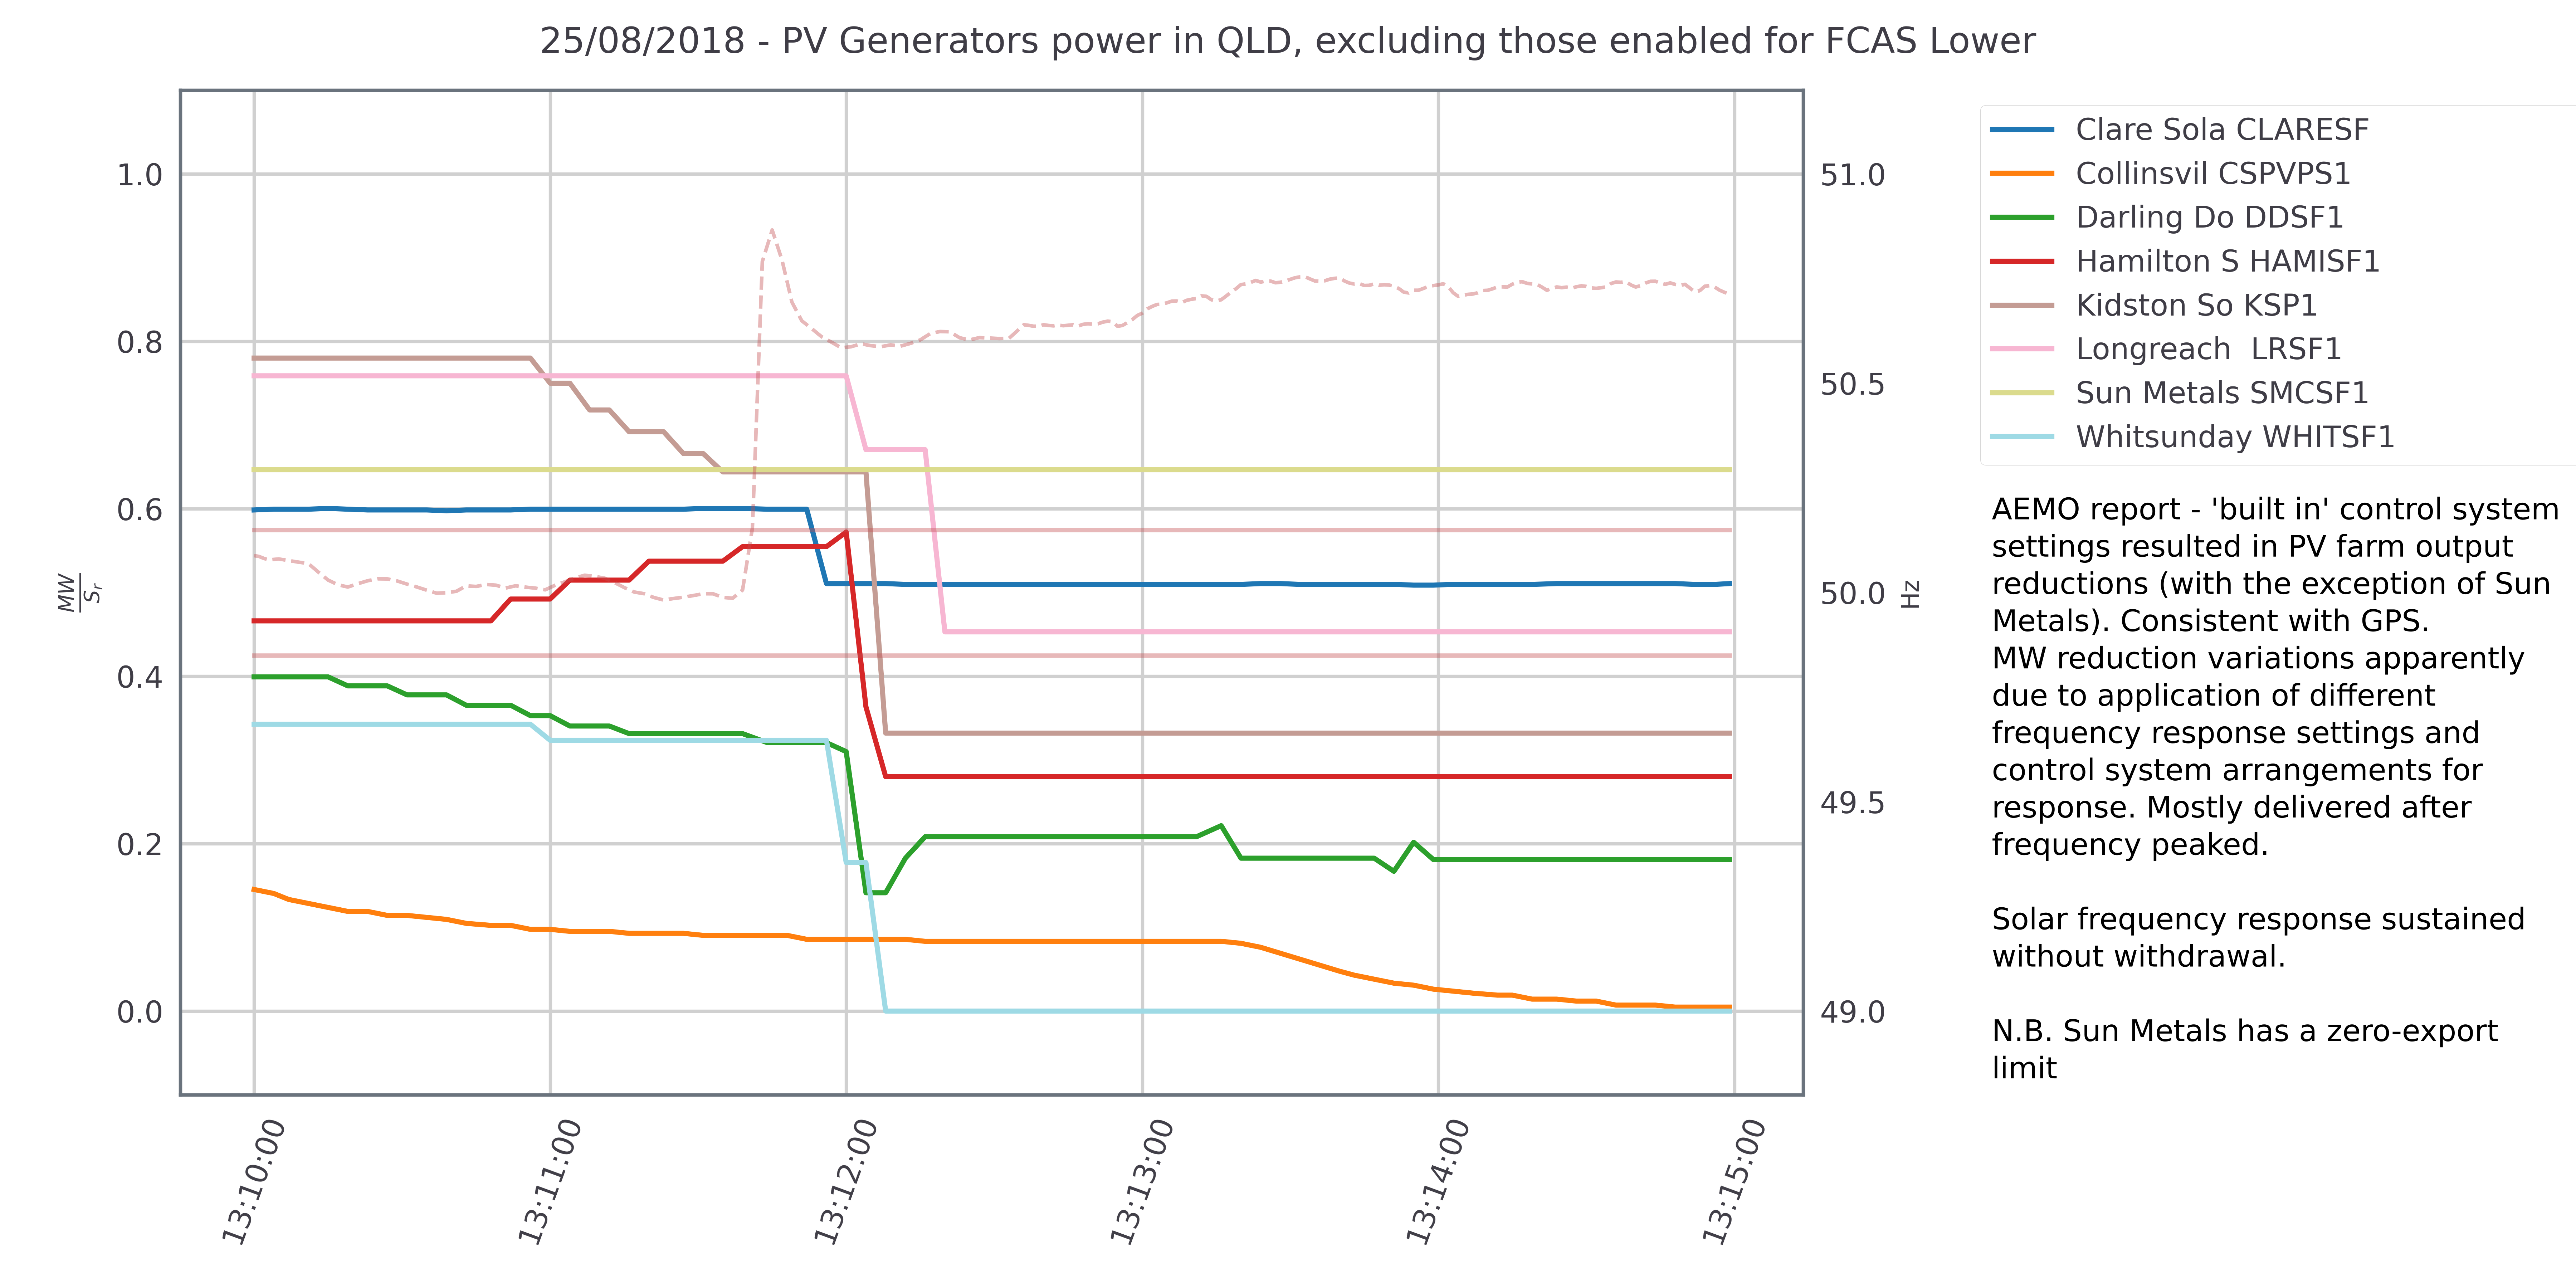
\includegraphics[width=\linewidth]{figures/QLD_PV_PU_annotated.png}
    \label{fig:qld_pv}
\end{figure}

%  \note{
%     This slide has notes too.
%   }

\end{frame}

\begin{frame}{GTPS for Connection after 5/10/2018}
\begin{itemize}
\item Schedule 5.2.5 of NER includes GTPS for connection
    \begin{itemize}
    \item \textbf{S5.2.5.3} - Response to frequency disturbance
    \begin{itemize}
        \item MAS & AAS - Minimum ride-through times for various frequency bands
    \end{itemize}
    \item \textbf{S5.2.5.8} - Protection from disturbances
    \begin{itemize}
        \item MAS - Facilities to automatically and rapidly reduce output by at least half if frequency exceeds level nominated by AEMO (not less than upper limit of OFTB - $\pm$ 1 Hz)
    \end{itemize}
    \item \textbf{S5.2.5.11} - Frequency control
    \begin{itemize}
        \item MAS - not work against frequency control and \textit{capability} of operating in frequency response mode
        \item AAS - not work against frequency control and \textit{capability} of operating in frequency response mode such that could provide all FCAS services
        \item Frequency response mode must automatically provide proportional response
    \end{itemize}
    \end{itemize}
\end{itemize}
\end{frame}
\end{document}
